\let\negmedspace\undefined
\let\negthickspace\undefined
\documentclass[journal]{IEEEtran}
\usepackage[a5paper, margin=10mm, onecolumn]{geometry}
%\usepackage{lmodern} 
\usepackage{tfrupee} 

\setlength{\headheight}{1cm} 
\setlength{\headsep}{0mm}     

\usepackage{gvv-book}
\usepackage{gvv}
\usepackage{cite}
\usepackage{amsmath,amssymb,amsfonts,amsthm}
\usepackage{algorithmic}
\usepackage{graphicx}
\usepackage{textcomp}
\usepackage{xcolor}
\usepackage{txfonts}
\usepackage{listings}
\usepackage{enumitem}
\usepackage{mathtools}
\usepackage{gensymb}
\usepackage{comment}
\usepackage[breaklinks=true]{hyperref}
\usepackage{tkz-euclide} 
\usepackage{listings}                                        
\def\inputGnumericTable{}                                 
\usepackage[latin1]{inputenc}                                
\usepackage{color}                                            
\usepackage{array}                                            
\usepackage{longtable}                                       
\usepackage{calc}                                             
\usepackage{multirow}                                         
\usepackage{hhline}                                           
\usepackage{ifthen}                                           
\usepackage{lscape}

\begin{document}

\bibliographystyle{IEEEtran}
\vspace{3cm}

\title{4.3.9}
\author{AI25BTECH11003 - Bhavesh Gaikwad}
{\let\newpage\relax\maketitle}

\renewcommand{\thefigure}{\theenumi}
\renewcommand{\thetable}{\theenumi}
\setlength{\intextsep}{10pt} 


\numberwithin{equation}{enumi}
\numberwithin{figure}{enumi}
\renewcommand{\thetable}{\theenumi}


\textbf{Question}: The vector equation of the line $\dfrac{x-5}{3} = \dfrac{y+4}{7} = \dfrac{z-6}{2}$ is?

\textbf{Solution:}\\
Given: 
\begin{equation}
\dfrac{x-5}{3} = \dfrac{y+4}{7} = \dfrac{z-6}{2}
\end{equation}
Let $\vec{A}$ be the parallel vector of the given line.\\
Let $\vec{B}$ be the position vector of a point on the given line.\\

From Equation 0.1,
\begin{equation}
    \vec{A} = \myvec{3 \\ 7 \\ 2}
\end{equation}

Putting x=8 in Equation 0.1 to get an arbitrary point on the line,
\begin{equation}
\dfrac{8-5}{3} = \dfrac{y+4}{7} = \dfrac{z-6}{2}
\quad \Rightarrow x=8, \, y = 3, \, z=8.
\end{equation}

\begin{equation}
    \therefore \, \vec{B} = \myvec{8 \\ 3 \\ 8}
\end{equation}

From Equations 0.1 and 0.4,\\
The Vector Equation of the given line is: 
\begin{equation}
\vec{L} = \vec{B} + k\vec{A}    
\text{, Where } k \text{ is a real parameter OR } k \, \epsilon \, \mathbb{R}
\end{equation}


\begin{equation}
\boxed{\vec{L} =\myvec{8 \\ 3 \\ 8} +  k\myvec{3 \\ 7 \\ 2}}
\end{equation}


\begin{figure}[htbp]
    \centering
    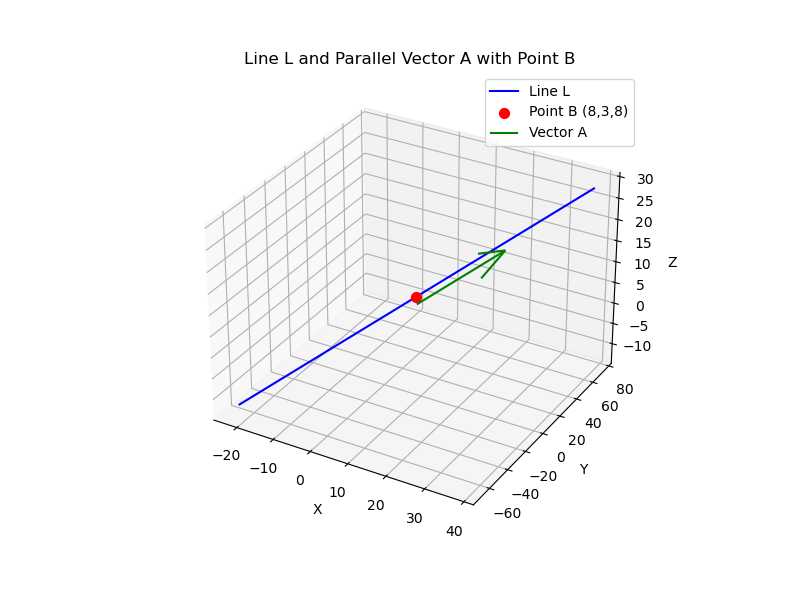
\includegraphics[width=\columnwidth]{figs/fig1.png}
    \caption{Line}
    \label{fig:fig/fig1.png}
\end{figure}
\end{document}  
